%!LW recipe=latexmk (XeLaTeX)
\documentclass[12pt,hyperref,a4paper,UTF8]{ctexart}
\usepackage{SJTUReport}
\usepackage{booktabs} % 三线表
\usepackage{amsmath} 

%%-------------------------------正文开始---------------------------%%
\begin{document}

%%-----------------------封面--------------------%%
% \cover

%%------------------摘要-------------%%
%\begin{abstract}
%
%在此填写摘要内容
%
%\end{abstract}

\thispagestyle{empty} % 首页不显示页码

%%--------------------------目录页------------------------%%
\newpage
\tableofcontents

%%------------------------正文页从这里开始-------------------%
\newpage

%%可选择这里也放一个标题
%\begin{center}
%    \title{ \Huge \textbf{{标题}}}
%\end{center}

\section{MPC模型建立}

\subsection{场景设置}

\begin{figure}[!htbp]
    \centering
    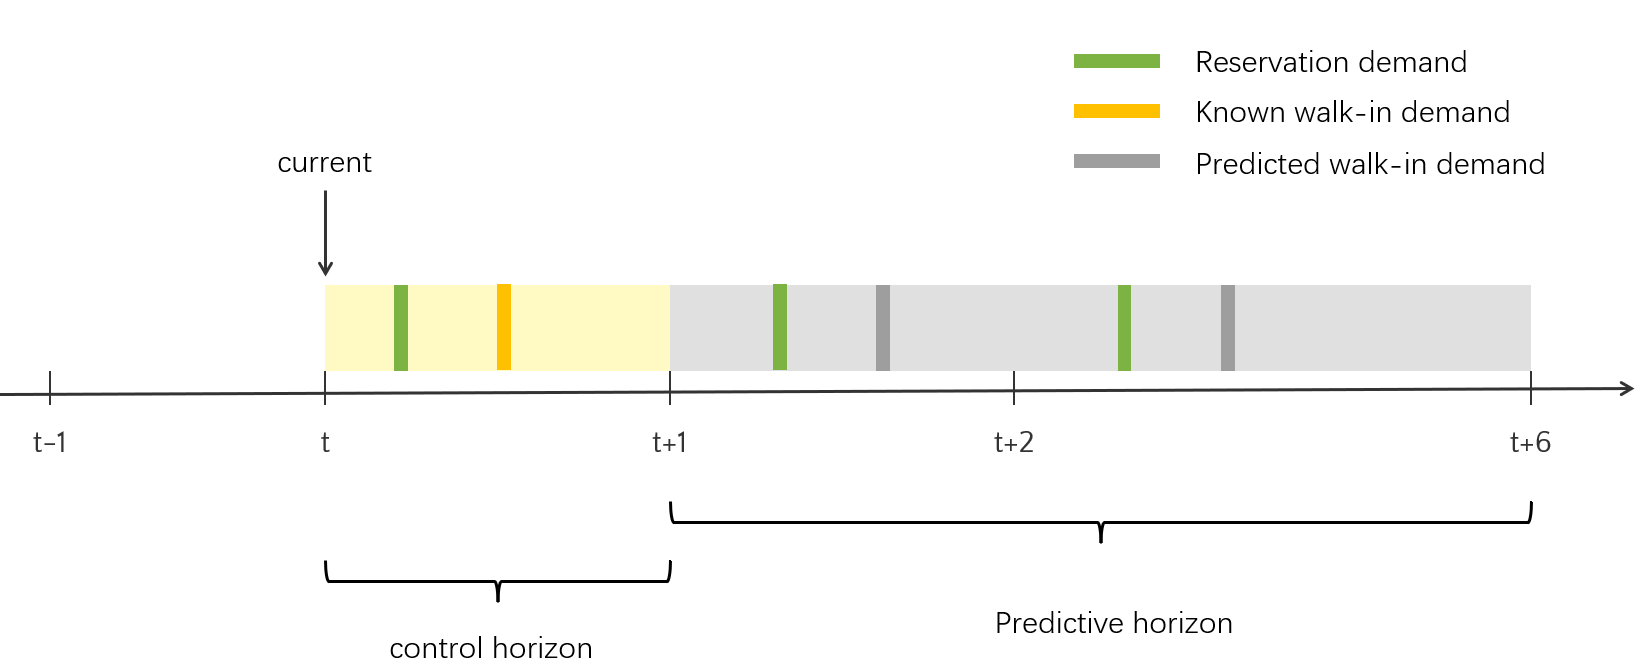
\includegraphics[width =1.0
    \textwidth]{figures/time_line.png}
    \caption{Rolling Horizon}
    \label{fig:Rolling Horizon}
\end{figure}

在t时刻，做出决策t+1时段的预约用户分配决策。

是否应该硬性保证每个预约用户都能得到服务？

\begin{itemize}
    \item 如果不硬性保证每个预约用户都能得到服务，那么存在一个风险，就是用户凭什么要预约，以及按照指派？ 在建模中使得预约用户优先级高于walk-in用户。更容易保证得到服务。或者调高惩罚参数，使得保证99\%的服务率。
    \item 如果硬性保证每个成功预约的用户都能得到服务，必须提前设置预约限制。预约限制如何设置也是一个问题。
\end{itemize}

\subsection{变量列表}

本文使用的变量如\autoref{tab:notation}所示。

% 导言区需确保已加载：
% \usepackage{booktabs}
% \usepackage{array}  % 推荐加载，增强表格功能

\begin{table}[!htbp]
  \centering
  \caption{Notation table}
  \label{tab:notation}
  \small
  \begin{tabular}{@{}lp{12cm}@{}}
    \toprule
    \textbf{Notation} & \textbf{Description} \\
    \midrule
    \multicolumn{2}{l}{\textit{Sets and Indices}} \\
    $\mathcal{P}$ & Set of O-D pairs, indexed by $p$\\
    $\mathcal{T}$ & Set of time periods in predictive horizon, indexed by $t$ \\
    $\mathcal{N}$ & Set of charging state of batteries, $\mathcal{N}:=\{0,\dots,N\}$, indexed by $n$\\
    $\mathcal{B}$ & Set of batteries in each station, indexed by $b$ \\
    $\mathcal{S}^p$ & Set of intermediate BSSs passed through O-D pair $p$, indexed by $i, j$ \\
    $\mathcal{S}$ & Set of all BSSs in the system, $\mathcal{S}$:=$\bigcup_{p \in \mathcal{P}}\mathcal{S}^p$\\
    $\mathcal{V}^p$ & Set of nodes consisting of origin $o^p$, destination $d^p$, and all BSS $\mathcal{S}^p$ on the path of O-D pair $p$ \\  
    $\mathcal{A}^{n,p}$ & Set of arcs in battery swapping network for original state $n$, O-D pair $p$ \\
    $\mathcal{G}^{n,p}$ & Directed graph for original state $n$, O-D pair $p$, $\mathcal{G}^{n,p}:=(\mathcal{V}^p,\mathcal{A}^{n,p})$ \\
    $Path^p$ & Set of all possible paths from origin to destination for O-D pair $p$ \\
    \midrule
    \multicolumn{2}{l}{\textit{Parameters}} \\
    % $s^q$ & Origin node of demand flow $q$ \\
    % $r^q$ & Destination node of demand flow $q$ \\
    $R$ & Driving range \\
    % R^L$ & Driving range of long-range battery (km) \\
    % $N^b$ & Number of time periods required to fully charge a battery of type $b$\\
    % $N^l$ & Number of time periods required to fully charge a long-range battery \\
    $M_i$ & Number of available charging slots at station $i$ \\
    $\tau_{p,i,t}$ & The travel time of the EV departing at time $t$ arriving to station $i$ for O-D pair $p$\\
    $\tau_{p,max}$ & The maximum travel time of the EV for O-D pair $p$\\
    $P_{b,i,t}$ & Charging power of each battery $b$ in station $i$ in time period $t$\\
    $e_{i,t}$ & Electricity price at station $i$ in time period $t$\\
    $s_{i,t}$ & Service fee for battery swap of type $b$ at station $i$ in time period $t$\\
    $v^{n,p}_{i,j}$ & The amount of electricity consumed by an appointed EV with an initial charging state $n$ from station $i$ to $j$ for O-D pair $p$\\
    $v^{n}_{i}$ & The amount of electricity consumed by a walk-in EV with an initial charging state $n$ arriving at station $i$\\
    % $SOC_{b,i,t}$ & soc of battery $b$ at station $i$ in time period $t$ \\ 
    % $P_t^L$ & Service fee for long-range battery swap at time $t\in\mathcal{T}$\\
    % $P^C$ & Compensation for long-range customers swapping to standard-range battery\\
    % $c^b$ & Unit temporary configuration cost of batteries of type $b$ \\
    % $c^L$ & Unit cost of long-range battery (currency) \\
    $x_i^b$ & Initial number of batteries at station $i$ \\
    % $\hat{x}_i^L$ & Initial number of long-range batteries at station $i$ \\
    % $\bar{I}$ & Maximum battery inventory limit at each station \\
    $\alpha$ & Penalty cost per unit of unsatisfied reservation demand\\
    $f_A^{n,p,t}$ & Reservation demand volume of EVs in original state $n$ for O-D pair $p$ at time $t$ \\
    $f_{R}^{n,i,t}$ & Random demand volume of EVs in original state $n$ at station $i$ in time period $t$ \\
    % $f_{\xi}^{L,q,t}$ & Demand volume of long-range EVs for flow $q$ at time $t$ under scenario $\xi$ \\
    \midrule
    \multicolumn{2}{l}{\textit{Variables}} \\
    % $x_i^b$ & Number of batteries of type $b$ allocated at station $i$ \\
    % $x_i^L$ & Number of long-range batteries allocated at station $i$ \\
    $y_{A,i,j}^{n,p,t}$ & Service volume of demand volume $f_{A}^{n,p,t}$ on arc $(i,j) \in A^{n,p}$ \\
    $y_{R}^{n,i,t}$ & Service volume of random demand volume $f_{R}^{n,i,t}$\\
    % $y_{i,j}^{L,q,t}$ & Service flow volume of long-range demand $f^{L,q,t}$ on arc $(i,j) \in A^{L,q}$ \\
    % $\hat{y}_{i,j}^{b,q,t}$ & Service volume of demand volume $f_{\xi}^{b,q,t}$ on arc $(i,j) \in A^{\bar{b},q}$, where $\bar{b}$ represents another battery type \\
    % $\hat{y}_{i,j}^{L,q,t}$ & Service flow volume of long-range demand $f^{L,q,t}$ on arc $(i,j) \in A^{S,q}$ (flexible swap) \\
    $w_{n,i,t}$ & Number of batteries in charging state $n$ at station $i$ in time period $t$ \\
    % $w_{t,n}^{l,i}$ & Number of long-range batteries at station $i$ that have been charged for $n$ periods at time $t$ \\
    % $z_{t,n}^{b,i}$ & Number of stage $n$ batteries of type $b$ at station $i$ being charged at time $t$. \\
    % $z_{t,n}^{l,i}$ & Number of long-range batteries at station $i$ being charged during period $t$ that have been charged for $n$ periods \\
    \bottomrule
  \end{tabular}
\end{table}


\subsection{soc-wised expanded network}
本文在expanded network的基础上，提出了soc-wised expanded network 建模方法，来表征不同初始SOC下的换电网络

\subsection{mathematical model}
目标函数：max 服务收益-用户用电成本-未满足惩罚-电站充电成本
\begin{equation}
max \quad I-C_1-C_2
\end{equation}

1. 服务收益 = （预约用户+随机用户）* 服务费

\begin{equation}
I=\sum_{t \in \mathcal{T}}  \sum_{n \in \mathcal{N}} 
\left[  
% y_{A,i,j}^{n,p,t} v_{i,j}s_{i,k} + y_{R}^{n,i,t}v_is_{i,t}
% \sum_{\{k\in\mathcal{T}|k+\tau_{p,i,k}=t\}}{y^{n,p,k}_{A,i,j}}
\sum_{p \in \mathcal{P}} 
\sum_{\{(i,j) | (i,j) \in \mathcal{A}^{n,p}\}} 
\left ( y^{n,p,t+\tau_{p,i,t}}_{A,i,j}v^{n}_{i,j}s_{i,t+\tau_{p,i,t}} \right )
+\sum_{i \in \mathcal{S}} y_{R}^{n,i,t}v^n_is_{i,t}
\right]
\end{equation}

% \begin{equation}
% I=\sum_{t \in \mathcal{T}}  \sum_{n \in \mathcal{N}} 
% \left[  
% % y_{A,i,j}^{n,p,t} v_{i,j}s_{i,k} + y_{R}^{n,i,t}v_is_{i,t}
% % \sum_{\{k\in\mathcal{T}|k+\tau_{p,i,k}=t\}}{y^{n,p,k}_{A,i,j}}
% \sum_{p \in \mathcal{P}} \sum_{\{(i,j) | (i,j) \in \mathcal{A}^{n,p}\}} \sum_{\{k\in\mathcal{T}|k+\tau_{p,i,k}=t\}} \left ( y^{n,p,k}_{A,i,j}v^{n}_{i,j}s_{i,t} \right )
% +\sum_{i \in \mathcal{S}} y_{R}^{n,i,t}v^n_is_{i,t}
% \right]
% \end{equation}

% 2. 用户用电成本 = （预约用户+随机用户）* 分时用电成本
% \begin{equation}
% C_1=\sum_{t \in \mathcal{T}}  \sum_{n \in \mathcal{N}} 
% \left[  
% \sum_{p \in \mathcal{P}} \sum_{\{(i,j) | (i,j) \in \mathcal{A}^{n,p}\}} \sum_{\{k\in\mathcal{T}|k+\tau_{p,i,k}=t\}} \left ( y^{n,p,k}_{A,i,j}v^{n,p}_{i,j}e_{i,t} \right )
% +\sum_{i \in \mathcal{S}} y_{R}^{n,i,t}v^n_ie_{i,t}
% \right]
% \end{equation}

2. 未满足惩罚 = 预约用户 * 未满足惩罚
\begin{equation}
C_1 = \alpha \sum_{t\in \mathcal{T}} \sum_{p\in \mathcal{P}}  \sum_{n\in \mathcal{N}} 
\left[
f^{n,p,t}_A - \sum_{\{j | (o^p,j) \in \mathcal{A}^{n,p}\}} y^{n,p,t}_{A,o^p,j} \right]
\label{eq:penaltycost}
\end{equation}

3. 电站充电成本 = 每个站点每种规格的正在充电的电池数量*对应功率*电价
\begin{equation}
C_2 = \sum_{t \in \mathcal{T}}  \sum_{n \in \mathcal{N}} \sum_{i \in \mathcal{S}}
\left[
w_{n,i,t}P_{n,i,t}e_{i,t}
\right]
\end{equation}

约束条件：

1. 流平衡约束
\begin{subequations}
\label{eq:flow}
\begin{gather}
\sum_{\{j| (o^p,j)\in \mathcal{A}^{n,p}\}}{y^{n,p,t}_{o^p,j}} \leq f^{n,p,t}_A,\quad \forall{p\in \mathcal{P},t\in \mathcal{T}},n \in \mathcal{N}\label{eq:flow1}\\
\sum_{\{j| (i,j)\in \mathcal{A}^{n,p}\}}{y^{n,p,t}_{i,j}} =\sum_{\{j| (j,i)\in \mathcal{A}^{n,p}\}}{y^{n,p,t}_{j,i}},\quad \forall{p\in \mathcal{P},t\in \mathcal{T},i\in \mathcal{S}^p}\label{eq:flow2}
\end{gather}
\end{subequations}

2. 电池状态转移约束
对soc r<N 的电池状态转移约束：

i电站t时刻soc为r的电池 = t时刻到达电站i且soc为r的预约和随机用户+t时刻充到r的电池数

t时刻充到r的电池数 = count (前面所有的电池+功率 == r )


\begin{equation}
\begin{aligned}
w_{r,i,t}
=&
\sum_{p\in P}
\sum_{n\in N}
\sum_{\{j\mid (j,i)\in A^{n,p}\}}
\sum_{\{k\in T\cup\{-\tau_{p,max},...,0\}\mid k+\tau_{p,i,k}=t\}}
y^{n,p,k}_{A,j,i}
\mathbb{I}\!\left(N-v^{n,p}_{j,i}=r\right)
\\
&+
y^{r,i,t}_{R}
+
\sum_{m\in N}
w_{m,i,t-1}
\mathbb{I}\!\left(m+P_{m,i,t-1}=r\right),
\\
&\forall i\in S,\ r\in \mathcal{N}\setminus\{N\},\ t\in \mathcal{T}\setminus\{0\}.
\end{aligned}
\tag{7a}
\end{equation}

$\mathbb{I}\!\left(N-v^{n,p}_{j,i}=r\right)$
表示预约用户在电站 i 退回的电池 SOC 为 r。

$\mathbb{I}\!\left(m+P_{m,i,t-1}=r\right)$
表示上一时刻 SOC 为 m 的站内电池，经过充电后在时刻 t 变成 SOC 为 r 的电池。

对满电电池的状态转移约束：

\begin{equation}
\begin{aligned}
w_{N,i,t}
=&
\sum_{m\in N}
w_{m,i,t-1}
\mathbb{I}\!\left(m+P_{m,i,t-1}=N\right)
\\
&-
\sum_{p\in P}
\sum_{n\in N}
\sum_{\{j\mid (i,j)\in A^{n,p}\}}
\sum_{\{k\in T\cup\{-\tau_{p,max},...,0\}\mid k+\tau_{p,i,k}=t\}}
y^{n,p,k}_{A,i,j}
\\
&-
\sum_{n\in N}
y^{n,i,t}_{R},
\\
&\forall i\in S,\ t\in T\setminus\{0\}.
\end{aligned}
\tag{7b}
\end{equation}

i电站t时刻soc为N的电池 = t时刻充到N的电池数 - 换走的电池数

t时刻充到N的电池数 = count (前面所有的电池+功率 == N )

换走的电池数 = t时刻到达电站i的预约和随机用户

% \begin{subequations}
% \label{eq:transition}
% \begin{gather}
% \end{gather}
% \end{subequations}

3. 换电过程约束

由于换电站仅向用户提供满电电池，因此时刻 $t$ 电站 $i$ 可用于换电的满电电池数量为上一时刻站内电池经过充电后达到满电状态的电池数量。预约用户具有优先服务权，随机用户只能使用预约用户换电后剩余的满电电池。

\begin{align}
\sum_{n\in N} y^{n,i,t}_{R}
&\le
\left[
\sum_{m\in N} w_{m,i,t-1}
\mathbf{1}\!\left(m+P_{m,i,t-1}=N\right)
-
\sum_{p\in P}
\sum_{n\in N}
\sum_{\{j\mid (j,i)\in A^{n,p}\}}
\sum_{\{k\in T\cup\{-\tau_{p,max},...,0\}\mid k+\tau_{p,i,k}=t\}}
y^{n,p,k}_{A,j,i}
\right]^+, \notag \\  % 第一行不编号
&\quad \forall i\in S,\ t\in T\setminus\{0\}.
\tag{8a}
\end{align}

其中，$\sum_{m\in N} w_{m,i,t-1}\mathbf{1}(m+P_{m,i,t-1}=N)$ 表示时刻 $t$ 电站 $i$ 可用于换电的满电电池数量；
$\sum_{p\in P}
\sum_{n\in N}
\sum_{\{j\mid (j,i)\in A^{n,p}\}}
\sum_{\{k\in T\cup\{-\tau_{p,max},...,0\}\mid k+\tau_{p,i,k}=t\}}
y^{n,p,k}_{A,j,i}$ 表示时刻 $t$ 到达电站 $i$ 并需要换电的预约用户需求量。
该约束表示预约用户优先占用可用满电电池，随机步入用户只能使用预约用户占用后的剩余满电电池。当满电电池数量不足以满足预约用户需求时，右端为零，随机步入用户不能被服务，从而保证预约用户的优先服务权。


\begin{equation}
0\le y^{n,i,t}_{R}\le f^{n,i,t}_{R},
\qquad
\forall i\in S,\ n\in N,\ t\in T.
\tag{8b}
\end{equation}

这里 (8a) 保证预约用户优先占用满电电池，(8b) 保证随机用户服务量不超过实际随机需求量。


4. 边界条件约束


为保证电池状态转移约束在时间边界和 SOC 边界处定义良好，设置如下边界条件。

首先，给定各电站在初始时刻的电池 SOC 分布：
\begin{equation}
w_{n,i,0}=\bar{w}_{n,i,0},
\quad \forall n\in N,\ i\in S.
\tag{9a}
\end{equation}

其中，$\bar{w}_{n,i,0}$ 表示初始时刻电站 $i$ 中 SOC 状态为 $n$ 的电池数量。
该约束用于初始化电池库存状态，使得后续时段的电池状态转移约束可以从 $t=0$ 开始递推。

其次，所有服务量和电池库存变量均应满足非负性约束：
\begin{equation}
w_{n,i,t}\ge 0,
\quad \forall n\in N,\ i\in S,\ t\in T,
\tag{9b}
\end{equation}

\begin{equation}
y^{n,p,t}_{A,i,j}\ge 0,
\quad \forall p\in P,\ n\in N,\ t\in T,\ (i,j)\in A^{n,p},
\tag{9c}
\end{equation}

\begin{equation}
y^{n,i,t}_{R}\ge 0,
\quad \forall n\in N,\ i\in S,\ t\in T.
\tag{9d}
\end{equation}

若需求量和电池数量均以整数计，则进一步有：
\begin{equation}
w_{n,i,t},\ y^{n,p,t}_{A,i,j},\ y^{n,i,t}_{R}\in \mathbb{Z}_{+}.
\tag{9e}
\end{equation}



% 对于时间边界，仅允许在预测时域内完成的行程进入状态转移约束。若预约用户从电站 $i$ 出发的时间为 $k$，到达时间 $k+\tau_{p,i,k}$ 超出预测时域，则对应服务变量置为零：
% \begin{equation}
% y^{n,p,k}_{A,i,j}=0,
% \quad
% \forall p\in P,\ n\in N,\ (i,j)\in A^{n,p},\
% k\in T:\ k+\tau_{p,i,k}\notin T.
% \tag{9h}
% \end{equation}

% 该约束保证所有进入电池状态转移方程的到达流均发生在当前预测时域内，避免出现到达时间超出 $T$ 后无法更新电池库存的问题。

为避免 MPC 在预测时域末端过度消耗满电电池，设置终端库存约束：
\begin{equation}
w_{N,i,|T|-1}\ge \underline{w}_{N,i},
\quad \forall i\in S.
\tag{9i}
\end{equation}

其中，$\underline{w}_{N,i}$ 表示预测时域末端电站 $i$ 至少需要保留的满电电池数量。
该约束为可选约束，用于缓解有限预测时域导致的末端效应。

\section{写在最后}
\subsection{发布地址}
\begin{itemize}
    \item Github: 
    % \url{https://github.com/Jiazhen-Lei/SJTU_Course_Template_Latex}
\end{itemize}

%%----------- 参考文献 -------------------%%
%在reference.bib文件中填写参考文献，此处自动生成

\reference


\end{document}